\section{Design of \name}
% \begin{figure}[htbp]
%     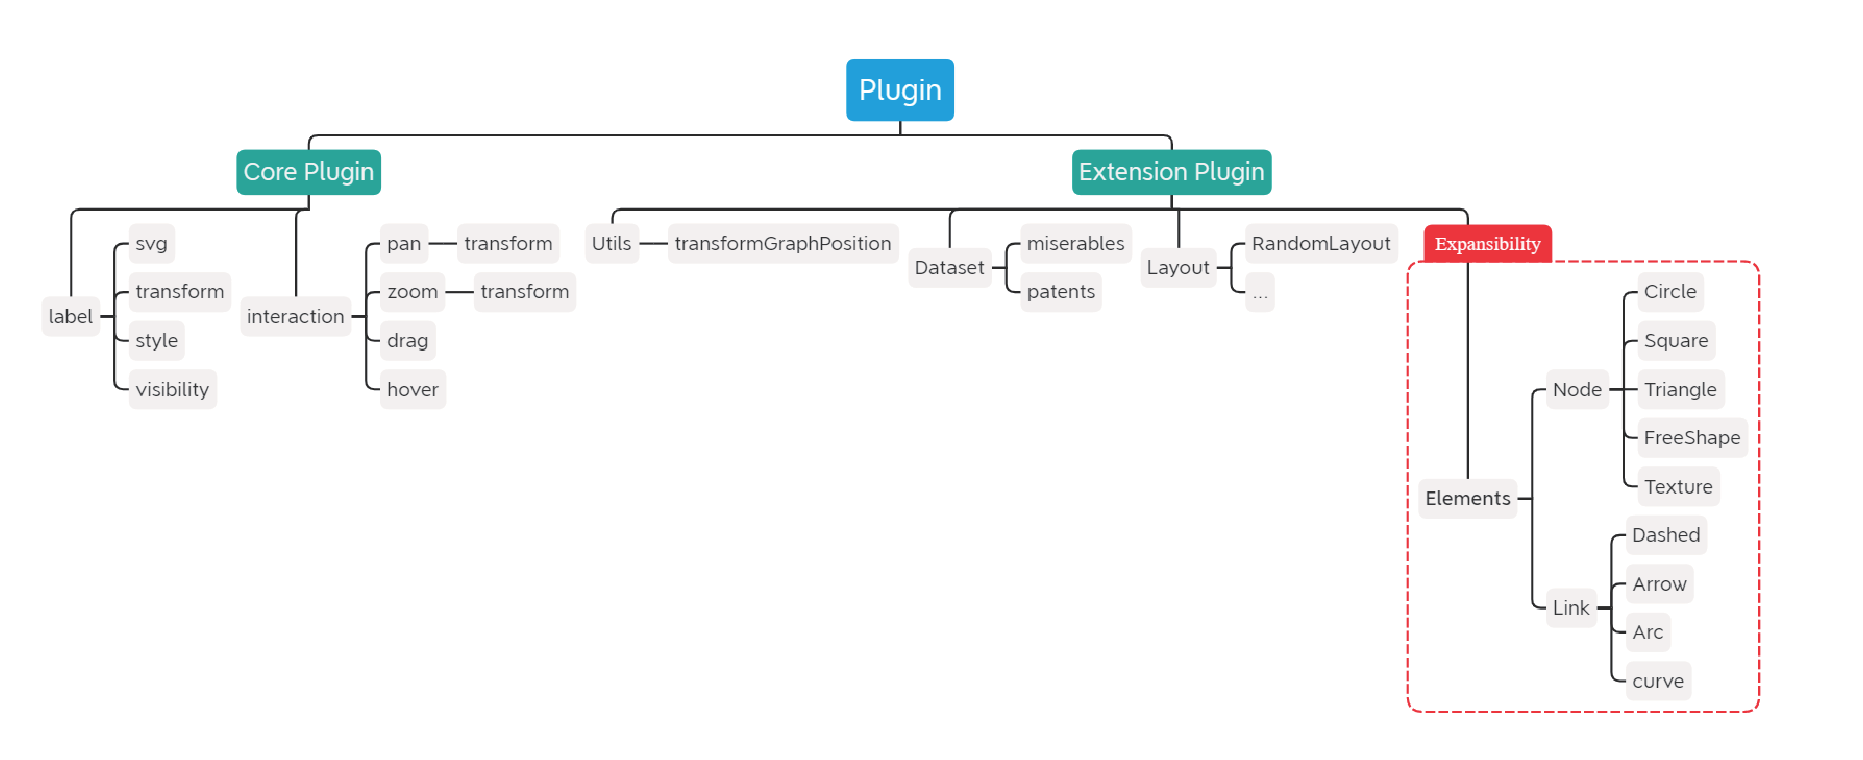
\includegraphics[width=\linewidth]{fig/xmind-02.eps}
%     \caption{
%         \name designs: \name consists of three parts: core engine, plugins, and library interface.
%     }
%     \label{fig:design}
% \end{figure}
% \begin{figure}[htbp]
%     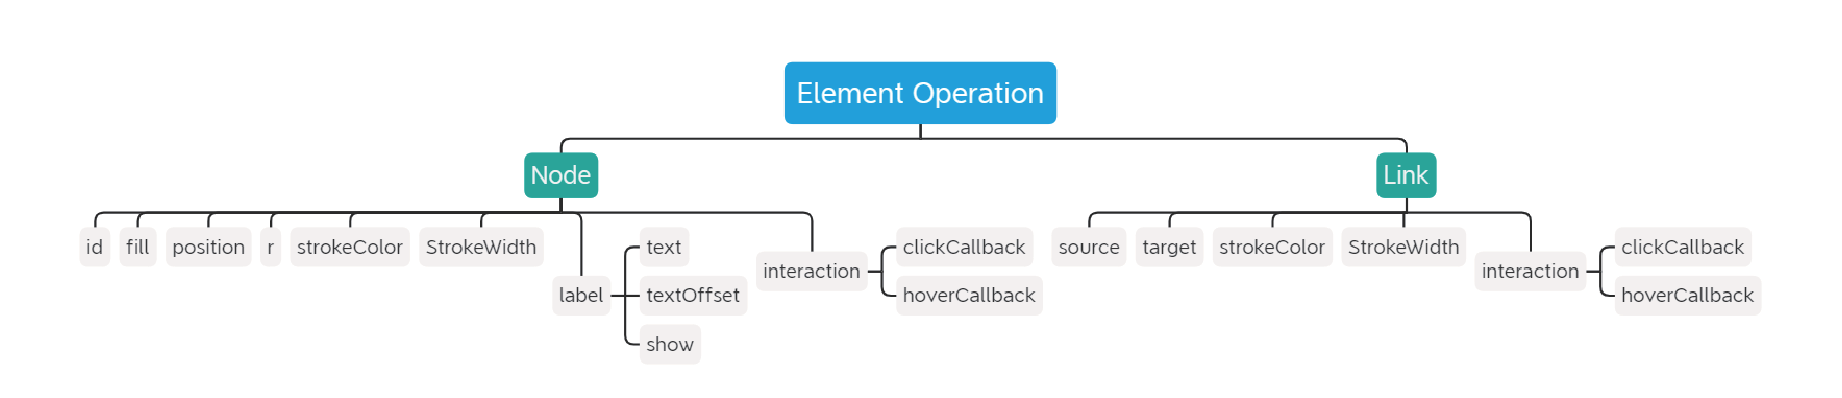
\includegraphics[width=\linewidth]{fig/xmind-03.eps}
%     \caption{
%         \name designs: \name consists of three parts: core engine, plugins, and library interface.
%     }
%     \label{fig:design}
% \end{figure}
% \begin{figure}[htbp]
%     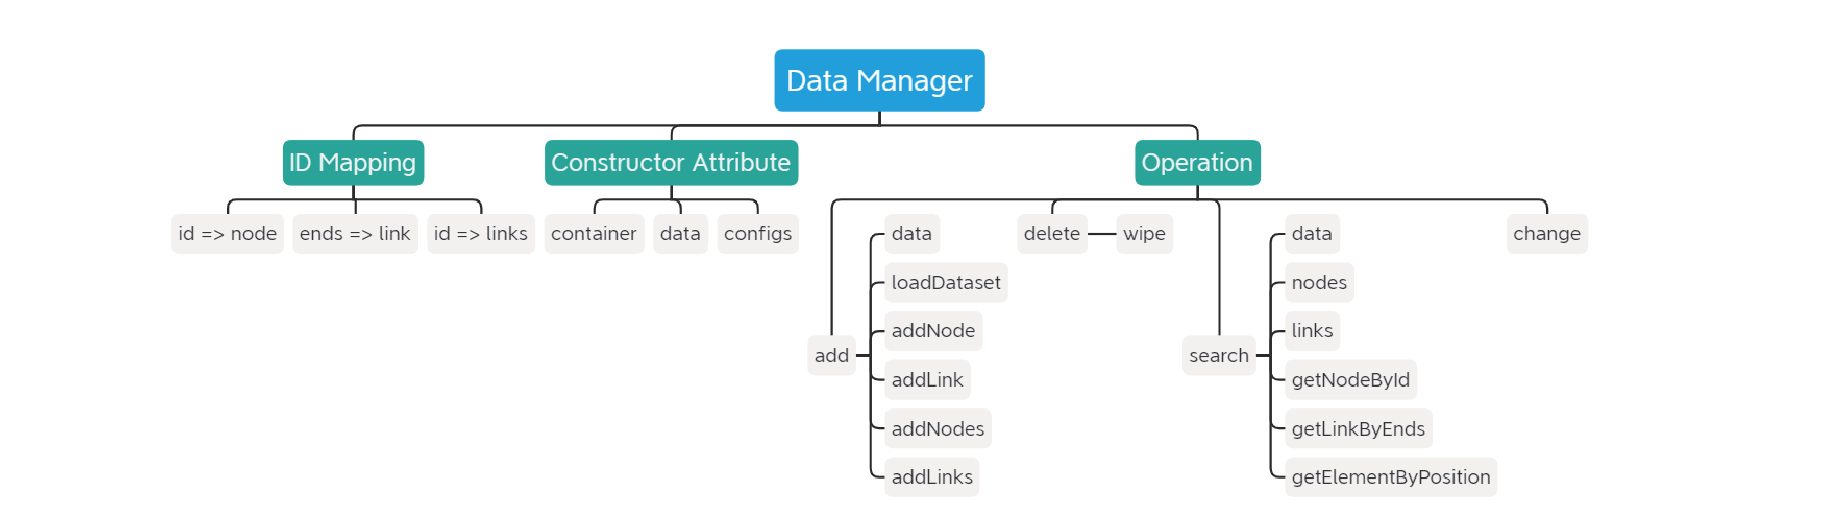
\includegraphics[width=\linewidth]{fig/xmind-04.eps}
%     \caption{
%         \name designs: \name consists of three parts: core engine, plugins, and library interface.
%     }
%     \label{fig:design}
% \end{figure}

\subsection {Design Requirements of \name}

\deleted[id=pan]{为了探索\name的设计空间,我们采访了3个图可视化相关的专家,调研了一系列图可视化的工具,包括 Gephi, Cytoscape.js, Sigma.js, GraphViZ,总结了如下高性能节点链接图可视化的设计需求:}

\added[id=pan] {
    To explore the design space of \name, we interviewed three graph visualization experts, investigated five graph visualization tools including Gephi~\cite{DBLP:conf/icwsm/BastianHJ09}, Cytoscape.js~\cite{DBLP:journals/bioinformatics/FranzLHDSB16}, SNAP~\cite{leskovec2016snap}, Sigma.js~\cite{DBLP:journals/jossw/Coene18}, and GraphViZ~\cite{Ellson03graphvizand}.
    We summarized the following design requirements for high-performance node-link diagram visualization: 
}

\begin{enumerate}[label*=\textbf{R\arabic*}] % \usepackage{enumitem}
\item \deleted[id=pan]{
    \textbf{需要有抽象的图模型来帮助控制图数据}: 在节点链接图中,可视化元素和图数据元素一一对应,开发者只需控制图数据元素,而并不需要直接访问图可视化元素。
    为了简化对于图数据和可视化的操作,开发者需要一个抽象图模型来控制图数据元素。该模型需要支持图的以下几点特性:}
    \added[id=pan]{
        \textbf{An abstract graph model to manipulate graph data}. 
        In a node-link diagram, visual elements (graphical marks) are one-to-one corresponding to data elements (nodes and links). 
        Developers only needs to manipulate graph data elements rather than to access visual elements. 
        To simplify the manipulation of origin data and visualization, developers need an abstract graph model. Several features should be supported:
    } \label{R:model}
\begin{enumerate}[label*=\textbf{.\arabic*}]
    \item \deleted[id=pan]{\textbf{链接关联节点}: 每条链接都会关联到两个节点是图结构最基本的特性,该特性使得绘制节点链接图可以不关心链接的位置,开发者可以专注于节点的位置修改,链接会相应联动。}
    \added[id=pan]{
        \textbf{The node-link connection}.
        The basic characteristic of graph is that each link connects two nodes. 
        Developers only need to focus on modifiying the position of nodes and ignore the position of links when drawing a node-link diagram. 
        The position of links should be automatically determined.
    }\label{R:connection}
    \item \deleted[id=pan]{\textbf{邻节点和邻接边的可访问性}: 图数据的另一个特点就是,节点和它的邻节点,邻接边之间的相互关联。我们在调研过程中发现,很多可视化系统中支持了高亮某个节点的邻接边和邻节点的交互。所有专家都一致同意为图模型增加邻节点和邻接边可访问功能的重要性。}
    \added[id=pan]{
        \textbf{The accessibility of neighbors}.
        Another characteristic of graph is the connections among one node to its neighbor nodes and neighbor links.
        We found that many graph visualization systems support highlighting neighbor nodes and links of the focused node.
        All three experts agreed with that the graph model needs to support a node to access its neighbors.
    } \label{R:neighbors}
    \item \deleted[id=pan]{
        \textbf{基本图论算法的支持}: 某些场景需要一些图论的基本算法,比如计算某些度量(如节点度数,节点centrality,图直径等)可以用来高亮POI,最短路算法可以帮助用户追溯两个节点之间的关联。
        专家们都一致同意图论算法对于可视化的重要性,但他们部分同意实现图论算法的必要性,其中一个专家认为该功能不属于可视化渲染库所关心的需求。
    }
    \added[id=pan]{
        \textbf{Basic graph theory algorithms}.
        Graph algorithms play important roles in some senarios. 
        For example, some importance measurements (e.g. node degree, node centrality) can be used to highlight POIs (points of interest) and shortest paths finding algorithms can help users to trace the association between two nodes. 
    }\label{R:algorithms}
\end{enumerate}

\item \deleted[id=pan]{
    \textbf{需要对拥有大量可视化元素的节点链接图提供高刷新率}: 刷新率影响用户体验,当刷新率降低时,用户会感觉到明显的卡顿,影响他们的mindmap。
    根据我们对三位图可视化专家的采访,他们认为【对超过10万元素的大规模图有30fps以上的渲染速度】才能认为其对大规模节点链接图提供了高性能渲染的能力。
} \added[id=pan]{
    \textbf{High frame rate for large-scale node-link diagrams}.
    The frame rate can affect the user experience. 
    The user interface will respond slowly or even stop responding with a low frame rate.
    Base on our interview with three experts, a rule of thumb for high-performance rendering is ``\textit{reaching 30 FPS (Frames Per Second) for rendering node-link diagrams with more than 100 thousand visual elements}''.
}\label{R:fps}

\item \deleted[id=pan]{
    \textbf{支持基本的节点和链接的样式}: 开发者往往需要在节点链接图上编码不同信息,虽然在大部分大规模图可视化案例中,圆形的节点和直线边最受欢迎,但仍然有很多节点链接图支持了不同形状的节点和不同样式的边。
    因此,为节点和链接赋予不同的形状和样式,能使得开发者有更多可以编码信息的空间。最常见的节点形状有圆形、方形、三角形等,而最常见的链接形状有直线、曲线等
} \added[id=pan] {
    \textbf{Basic styles for nodes and links}.
    Developers often needs to encode information on node-link diagrams such as encoding degree with node size.
    Although circular nodes and straight links are popular in large-scale node-link diagrams, there are also nodes and links with diverse shapes and styles.
    The most common node shapes includes circles, rectangles and triangles and the most common link shapes include straight lines and curves.
}\label{R:styles}

\item \deleted[id=pan]{
    \textbf{需要提供多种布局功能和自定义布局插件}:节点链接图对于布局的依赖程度不言而喻。
    \name 需要提供一些基础的节点链接图布局。
    因为布局算法的多样性,\name 还需能使开发者按照既定接口接入自定义布局。
} \added[id=pan] {
    \textbf{Layout algorithms}.
    The dependence of node-link diagrams on layouts is self-evident.
    Thus, \name should provide some basic layout algorithms.
    Because of the diversity of layout algorihtms, \name should provide interfaces for developers to customize their own layout algorihmts.
}\label{R:layout}

\item \deleted[id=pan]{
    \textbf{需要提供自定义标签渲染}:标签展示了节点和链接的基本信息。虽然在渲染大规模节点链接图时,为可视化元素赋予标签会导致visual clutter的问题,但开发者仍有可能采取某些策略来绘制部分节点的标签。所以,\name有必要提供标签绘制的接口。
} \added[id=pan] {
    \textbf { Custom labels }. 
    Labels show basic information of nodes and links.
    Although drawing labels for all elements can lead to visual clutter in large-scale node-link diagrams, developers may adopt some strategies to select a part of elements to draw their labels.
    \name should provide interfaces for developers to draw custom labels.
}\label{R:label}

\item \deleted[id=pan]{
    \textbf{需要提供基础交互}:根据我们的调研和专家访谈,我们发现交互基本上都可以被分解为对节点、链接以及画布的交互监听。
    应该支持一些鼠标事件比如鼠标进入,鼠标移动,鼠标移出,鼠标释放和鼠标按下,以便它们组成更复杂的交互,比如拖动。
    还需要实现对节点链接图的可视化元素的选择功能,比如lasso。
} \added[id=pan] {
    \textbf {Basic interactions}.
    Based on our interview with experts and investigation on graph visualization authoring systems, we found interactions of node-link diagrams can be  decomposed into interactions on nodes, links, and the canvas. 
    Mouse events like mouseover, mousemove, mouseout, mouseup and mousedown should be supported to construct more complex interactions such as dragging nodes.
    Selection interactions such as lasso should also be supported.
} \label{R:interactions}
\end{enumerate}

\subsection{Design Details of \name}
\newcommand{\RenEng}{\textit{Rendering Engine}\xspace}
\newcommand{\GraModMan}{\textit{Graph Model Manager}\xspace}
\newcommand{\IntMan}{\textit{Interaction Manager}\xspace}

\begin{figure*}[htbp]
    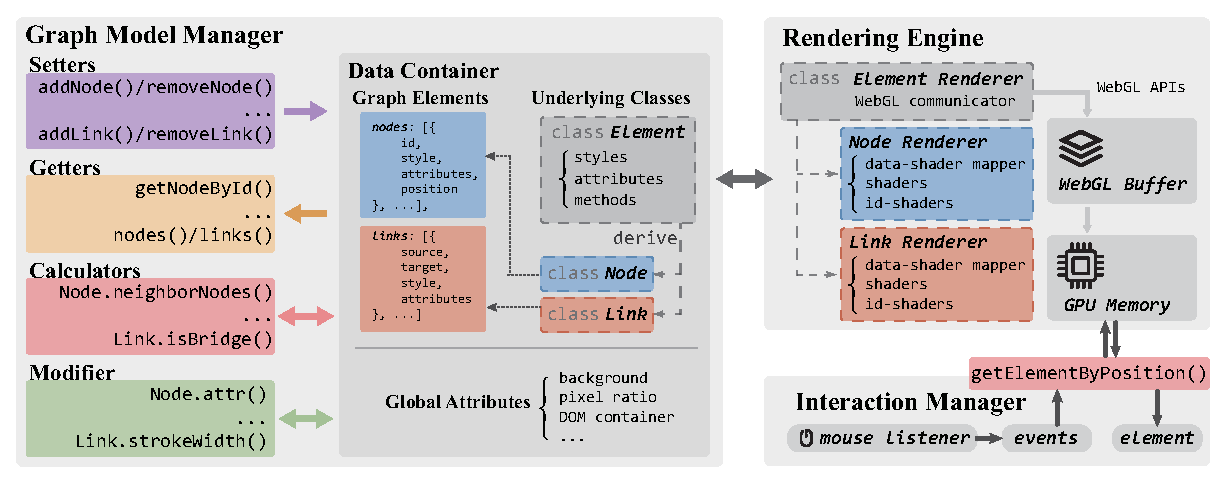
\includegraphics[width=\linewidth]{fig/architecture.eps}
    \caption{
        \name designs: \name consists of three main parts: (a) \GraModMan, (b) \RenEng, and (c) \IntMan.
    }
    \label{fig:design}
\end{figure*}

\deleted[id=pan]{
    为了完成上述的需求,我们设计实现了 \name。\name 包含了三个主要部分:\GraModMan 、\RenEng 以及 \IntMan (图\ref{fig:design})。
    我们还将其余的需求(\ref{R:layout}, \ref{R:label}, \ref{R:interactions})独立为插件的形式方便开发者自定义调用,从而减少\name的核心代码。
}

\added[id=pan] {
    To fullfill the proposed requirements, we designed and implemented \name. \name consists of three main parts: \GraModMan, \RenEng, and \IntMan (Figure~\ref{fig:design}).
    We isolate \ref{R:layout}, \ref{R:label}, and selection interactions (\ref{R:interactions}) into three different plugins to reduce the code length of \name.
}

\subsubsection{\GraModMan}
\deleted[id=pan]{
    为了帮助开发者统一管理数据和可视化,我们在\name中设计实现了\GraModMan。
    该控制器的主体是一个Data Container,其存储了节点数据和链接数据。
    每个节点拥有一个唯一标志符id,其对应的样式会被存储在style属性中,而位置坐标被存储在position中,其余的属性则会被存储在attributes中;
    同样的,每个link都拥有一个source和一个target,代表它所关联的两个节点,其对应的样式和其余属性会被存储在style和attributes中。
    我们为节点和链接建立了对应的class:Node和Link来存储每一个数据实体。他们派生自Element类。
}

\added[id=pan]{
    To help developers manipulate data and visualization in a unified way (\ref{R:model}), we designed \GraModMan in \name (Figure~\ref{fig:design}(a)).
    The core of \GraModMan is an \textit{Data Container}. It stores data elements including nodes and links.
    Each node contains a unique identifier (\codeword{id}).
    Its styles are stored in \codeword{style} attribute and coordinates are stored in \codeword{position} attribute.
    Other information is stored in \codeword{attributes}.
    Similarly, each link contains a \codeword{source} and a \codeword{target} which represent two nodes the link connects.
    Styles and other information are stored in \codeword{style} and \codeword{attributes} in the same.
    In \name, nodes and links are stored in objects instanced from classes \codeword{Node} and \codeword{Link}. They are derived from \codeword{Element}.
}

\deleted[id=pan]{
    我们为data elements (nodes和links) 设计了 增、删、改、查和计算的功能。
    开发者可以通过data setter来增加和删除elements,
    通过 data getter 则能用于查询element,
    通过 data modifier 修改数据的内容(如属性、样式等)。
    除此以外,我们还提供了部分常用的图计算的接口,因为该部分和可视化的关联并不紧密,我们只实现了部分功能,比如查询节点的邻节点(\ref{R:neighbors}),最短路径查找等 (\ref{R:algorithms})。\GraModMan 还可以管理一些整体的配置,比如 画布的背景颜色,DOM容器等等。
}

\added[id=pan]{
    We support developers to add, remove, modify, query and calculate data elements or visual elements. 
    \textit{Data Setters} are designed to add and remove data elements. 
    \textit{Data Getters} are designed to query elements (e.g. querying nodes by \codeword{id}s). 
    Developers can modify the style and attributes of elements through \textit{Data Modifier}.
    Several comman graph algorithms are supported in \name. Because they are not strongly related to graph visualization, we only implemented several interfaces such as neighbor nodes/links querying (\ref{R:neighbors}) and shortest paths fingding (\ref{R:algorithms}).
    Besides, \GraModMan can also manipulate global configurations such as backgrond color of the canvas and the DOM container.
}

\subsubsection{\RenEng}

\deleted[id=pan]{
    为了满足\textbf{\ref{R:fps}},\RenEng 调用了GPU的高性能渲染来绘制可视化。
    \RenEng 的主要工作流程是将节点和链接的样式以及位置,映射到 WebGL的 shader 程序中,通过WebGL API 将数据输入 WebGL Buffer,并绘制到屏幕上。
    如此,\RenEng 将数据传输到浏览器的CPU内存,最终到GPU内存。
}

\added[id=pan] {
    To fullfill \ref{R:fps}, \RenEng utilizes the high-performance rendering ability of GPU.
    The workflow of \RenEng consists of: 1) mapping styles and positions of elements into WebGL shader variables; 2) loading corresponding data into the WebGL buffer using WebGL APIs; 3) transfering data in the buffer into GPU memory and than drawing elements on the screen.
    In this way, \RenEng transfers data to the CPU memory of the browser, and the GPU memory in the end.
}

\deleted[id=pan] {
    我们采用了一种被动式的buffer修改策略:当开发者修改样式时,\GraModMan 不会主动访问 \RenEng 以修改WebGL buffer的内容,而仅仅将被修改的节点存到一段修改元素缓冲池。
    当开发者调用重绘制的API时,\RenEng 遍历所有缓存池的元素以获取样式,然后根据 数据-shader的映射表,将样式映射到对应的WebGL Buffer上进行覆盖。
    相对的主动式的buffer修改策略,\GraModMan 直接访问 \RenEng 以修改WebGL buffer的内容。
    这种策略的优点是比较直观,数据是正向流动的。
    但每次样式进行修改,\GraModMan 都会访问 \RenEng 的相关接口,导致调用栈加深,降低效率。
}

\added[id=pan] {
    We adapted a passive buffer modifying strategy: when developers modify styles of elements, \GraModMan will not call \RenEng to modify the WebGL buffer but stores the modified elements into a cache pool. When developers try to refresh the canvas, \RenEng will traverse elements in the cache pool to get related attributes and cover their corresponding buffer content.
    The relative strategy is to forwardly change the WebGL buffer when developers modify styles of elements. It is more intuitive because the data flows forward. But every time one element is modified, \GraModMan will call the related interface of \RenEng to change the buffer. It deepens the call stack and reduces the efficiency of rendering.
}

\deleted[id=pan] {为了解决\ref{R:connection},我们禁止了开发者直接修改link的位置,而是当开发者修改node的位置时,将该节点和其所有邻接边都放入缓冲池,后续则会同步修改邻接边的表现。}

\added[id=pan] {
    We forbid developers to modify the position of links directly (\ref{R:connection}), but links will be cached in to the pool when developers modify the position of their connected nodes. \RenEng will update the WebGL buffer of links when the canvas is refreshed.
}

\deleted[id=pan] {
    我们的 \RenEng 还为节点和链接增加了许多基础的样式来满足\ref{R:styles}。
    我们为节点设计了四种不同的形状,包括圆形,矩形,三角形和十字形。
    开发者可以控制圆形节点的半径,矩形节点的长款,三角形节点的三个顶点和十字形顶点的粗细和大小。
    所有形状的节点都可设置填充颜色、边框颜色和边框宽度。
    我们为链接设计了两种不同的形状,分别为直线和曲线。开发者可以控制曲线的曲率。所有的链接都可以设置颜色、宽度和虚线。
}

\added[id=pan] {
    \RenEng supports rendering several basic styles of nodes and links (\ref{R:styles}).
    Nodes can be rendered with four different shapes: circles, rectangles, triangles, and crosses.
    Developers can control the radius (\codeword{r}) of circular nodes , the \codeword{width} and the \codeword{height} of rectanglar nodes, the verteces (\codeword{vertexAlpha}, \codeword{vertexBeta}, and \codeword{vertexGamma}) of triangular nodes , and the \codeword{thickness} and the \codeword{size} of cross nodes.
    Developers can set fill color (\codeword{fill}), the border color (\codeword{strokeColor}) and the border width (\codeword{strokeWidth}) of all kinds of nodes.
    Two different links are supported (the straight line and the curve). Developers can control the \codeword{curveness} of curve edges.
    Both two kinds of links support setting the color (\codeword{strokeColor}), the width (\codeword{strokeWidth}), and the dash array (\codeword{dashInterval}).
}

\subsubsection{\IntMan} \label{sec:interaction manager}

\begin{figure}[htbp]
    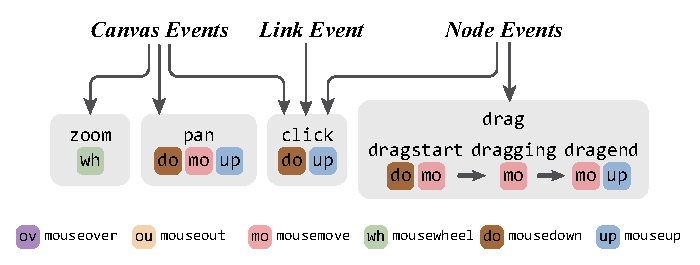
\includegraphics[width=\linewidth]{fig/interactions.eps}
    \caption{
        \name interactions decomposition. Canvas events include zoom, pan and click. Link event contains only click. And node events include click and drag.
    }
    \label{fig:interactions}
\end{figure}

\deleted[id=pan] {
    \IntMan 为 \name 提供了一系列基础的交互以满足\ref{R:interactions}。
    我们在画布上监听了鼠标的进入、离开、移动、按下、松开和滚动。
    通过不同事件的组合,我们实现了多种交互。
    例如,\name 通过监听和组合了鼠标滚动,鼠标按下,鼠标移动和鼠标松开,支持了zoom pan的交互。节点的拖动则可以被分解为拖动开始,拖动中,拖动结束。
    当用户在节点上按下鼠标,并开始移动鼠标时,就会触发拖动开始,接着拖动中被触发,当用户松开鼠标前,拖动结束会被触发,最后则触发鼠标松开事件。
}

\added[id=pan] {
    \IntMan provides a seriels of basic interactions (\ref{R:interactions}). 
    \name listens several mouse events (mouseover, mouseout, mousemove, mousedown, mouseup and mousewheel) on the canvas.
    All these events are supported on nodes, links and the canvas.
    We implemented several complex interactions by combining different events.
    For example, \name supports the zoom+pan interaction by listening and combining mousewheel, mousedown, mousemove, and mouseup. 
    Node dragging can be decomposed into several parts: dragstart, dragging, and dragend. 
    When users press the mouse and then move the mouse, dragstart will be triggered. Then dragging is triggered. When users release the mouse, dragend and mouseup are triggered one by one. 
    Figure~\ref{fig:interactions} shows events on nodes, links and the canvas.
}

\deleted[id=pan] {
    为了能够在屏幕上找出鼠标交互事件发生在哪个元素或者是画布上,我们在 \RenEng 中增加了一个隐藏层。
    该隐藏层将元素的唯一标志符编码到他们对应的像素上。
    于是,通过获知鼠标交互事件发生的屏幕像素的编码,我们就能获知交互的目标。
}

\added[id=pan] {
    To determine which element is interacted by the mouse, \RenEng generates a hidden canvas which encodes the unique identifiers of elements into their corresponding pixels.
    Developers can use the interface \codeword{getElementByPosition()} to get the identifier encoded on the mouse-focused pixel so that the element on the mouse-focused pixel can be gathered by developers immediately.
}


\subsubsection{Layout Plugin}

\deleted[id=pan]{
    节点链接图的可视化依赖布局算法为节点赋予相对位置。
    不同的布局算法调用接口不一,我们的插件为不同的布局算法提供统一的接口,方便开发者进行调用:
}

\added[id=pan]{
    Visualizing a node-link diagram relys on a layout algorithm to give the relative position of nodes.
    Different layout algorithms have different interfaces, our plugin intends to design a set of unified interfaces to facilate developer calling (\ref{R:layout}):
}

\begin{itemize}
    \item \deleted[id=pan]{
        调用开始接口能够让布局算法开始运行。为了提高性能,我们将布局算法实现为异步计算,为布局算法赋予独立的伪进程。
    } \added [id=pan]{
        \codeword{start()}: calling \codeword{start()} interface brings the algorithm into processing. To improve the frontend performance, \name creates another thread (using asynchronous timer) to calculate the layout result.
    }
    \item \deleted[id=pan]{调用结束接口能够让布局算法直接停止而不再进行后续的计算。} \added[id=pan] {
        \codeword{stop()}: calling \codeword{stop()} interface stops the layout thread immediately.
    }
    \item \deleted[id=pan]{
        调用onTick接口能够让开发者在回调函数中获取布局算法的每一步。
        一些布局算法并未提供布局的中间过程,我们尝试用差值函数来生成布局的中间过程,使得布局过程更加平滑。
    } \added[id=pan] {
        \codeword{onTick()}: calling \codeword{onTick()} enables developers to visit the intermediate status of the layout algorithm with its callback.
        Some layout algorithms do not provide intermediate status. \name generates intermediate status using interpolation functions. It make the layout process more smooth.
    }
    \item \deleted[id=pan] {
        调用onStop接口,能够在布局算法结束的一刻,让开发者获取到布局状态。
        结束并不一定是开发者调用了结束接口,也可能是布局算法运行结束。
    } \added[id=pan] {
        \codeword{onStop()}: calling \codeword{onStop()} raises the stopping status to developers and returns the layout result. It will be triggered when the algorithm finishes or developers call the \codeword{stop()} interface.
    }
\end{itemize}

\deleted[id=pan]{
    为了解决\ref{R:layout},我们在此标准上实现了径向层次布局算法和力引导算法。
    未来,我们将增加更多的布局算法方便开发者调用。
    开发者亦可以用这个标准接口实现自定义布局算法。
}

\added[id=pan] {
    To resolve \ref{R:layout}, we implemented a ratial tree layout and a force-directed layout based on these interfaces.
    In the future, we will increase more layout algorithms to facilate visualization.
    Developers can also implemente their own layout algorithms using our interfaces.
}

\subsubsection{Label Plugin}
\deleted[id=pan] {
    为了满足\ref{R:label},我们实现了Label Plugin。
    在大规模图渲染时绘制所有节点的标签会造成严重的视觉混乱,所以我们假设开发者只会渲染少数节点的标签,比如选取某些POI节点或区域绘制标签。
    于是我们选取了SVG作为标签的绘制工具,以提高可拓展性。
    除了默认的文本标签外,开发者还可以通过自己撰写标签模板来自定义标签。
}

\added[id=pan] {
    We implemented a label drawing plugin to facilate developers creating labels for elements (\ref{R:label}).
    When drawing a large-scale node-link diagram, drawing labels for all elements will cause serious visual clutter, so we assume that developers will only render labels for a few elements, for example, selecting some POI nodes or areas to draw labels.
    So we choosed SVG as label rendering tools to improve the expansibility.
    Besides the default textual label, developers can also customize labels by creating label templates.
}

\subsubsection{Selection Plugin}
\deleted[id=pan] {
    除了3.2.3章节提到的交互外,为了满足\ref{R:interactions},我们还实现了Selection Plugin,方便用户对图元素进行选取。
    常见的选择交互有框选和套索。
    因为套索的灵活性,我们选择了套索作为例子进行实现。
    开发者可以在套索的回调函数中获取到被选中的结构,包括节点和链接
    开发者可以通过配置来决定套索需要返回哪种元素。
}

\added{
    Besides interactions mentioned in Section \ref{sec:interaction manager}, we implemented a selection plugin to facilate elements selection.
    Common selection interactions include the box selection and the lasso selection.
    Because of the flexibility of the lasso selection, we implemente it for demonstration.
    Developers can get the selected structure (including nodes and links) in the callback function.
}


% % \name aims to help users rapidly and efficiently construct network visualization applications.
% % Specifically, \name consists of three parts: the core engine, plugins, and library interface (\autoref{fig:design}).
% % The core engine contains the data manager for maintaining nodes and links and the renderer for leveraging GPU processing power to render a large-scale network.
% % The plugins are employed to increase and expand more requirements and functions.
% % The library interface aims to help developers rapidly construct applications with friendly and concise APIs.


% % \subsection{Core Engine}
% % The core engine aims to render large-scale network based on WebGL and maintains the primary network information for rapidly editing operations.
% % It consists of the data manager and the renderer.

% % \subsubsection{Data Manager}
% % The data manager supports a series of interface corresponding network structure.
% % It is used to achieve nodes or links operations, including adding, deleting, searching, and editing.
% % Node-links and link-nodes mapping tables are also supported for accelerating search and locate.
% % At the same time, the data manager has a build-in network data set for developers to get started quickly.

% % \subsubsection{Renderer}
% % The renderer aims to render basic elements: nodes and links. It focuses on the efficiency of rendering massive data on the browser platform. As the highest performance graphics rendering API of browser platform, \name uses WebGL as the bottom rendering.
% % However, WebGL programming is still hard and complex.
% % The WebGL API is encapsulate
% % In order to reduce the program execution time as much as possible, the basic WebGL API is only encapsulated to meet the most basic data processing and rendering.
% % Specifically, the renderer uses three strategies to improve rendering efficiency.

% \begin{itemize}
% \item \textbf{Batch}: The renderer contains a batch drawing element instance. Considering that most of the elements of the network are the same, but the location information is different. The renderer creates an instance of an element and draws it in the batch process to reduce the consuming time of the rendering process.

% \item \textbf{Shader}: The renderer uses Shader function to control the shape render. Each node's shape usually needs to be defined as a circle, square, ellipse, and so on. However, the complex shape will cause a serious effect on rendering performance.
% \name exploits the powerful Shader function to define and render shape in GPU with batch processing.

% \item \textbf{Modify as needed}: The renderer supports manual rendering function for developers.
% The main attributes of elements, including positions, color, and texture, are stored into different buffers of GPU.
% When attributes of elements need to be Modified, the renderer can refresh corresponding buffers rather getting attributes from the data manager. And then, developers can refresh the network by supported function. The time consuming of getting attributes from the data manager can be omitted.

% \item \textbf{Element positioning}: The renderer has an elements positioning function for supporting elements search and interaction. For improving user interaction efficiency, the renderer uses the WebGL Texture to record the screen pixel position of each element.
% The time consuming of elements positioning has great improvement compared with index search and spatial index tree.
% The time complexity of the function is $O(1)$.

% \end{itemize}

% \subsection{Plugin module}
% The goal of the plugin modular is to enhance future expansions.
% For supporting more features and requirements, \name designs the plugin modular to employ new improvements or functions.
% At the same time, it can isolate the core modular from the rest.
% For now, the plugin module includes:
% \begin{itemize}
%     \item \textbf{Interaction: } It supports binding interaction events and callback functions of elements. Interaction events contain basis events of edges and nodes such as Hover, MouseDown, Click, etc.
%     \item \textbf{Layout: } It contains build-int layouts and allows users to use custom layouts.

% \end{itemize}

% \subsection{Library Interface}
% The library interface aims to support concise and efficient API for users to build large-scale network visual analysis applications quickly.
% Users do not need to touch the underlying WebGL rendering programming. Humanized and simple API can be called to config data and render network.
% Specifically, it includes three parts:
% \begin{itemize}
%     \item \textbf{Global: }It is used to define custom configs, such as the mount node, the default style of the canvas, and the default style of elements.
%     \item  \textbf{Element: }It includes the data adding of nodes of edges and the attributes changing of elements.
%     \item  \textbf{Plugin: }It aims to set up different plugins, such as layouts and interactions.
% \end{itemize}
